\documentclass[a4paper,12pt,french]{article}
\usepackage[margin=2cm]{geometry}
\usepackage[thinfonts]{uglix2}
\begin{document}
\titre{Réseaux et routage - RIP}{NSI2}{2023} 
\begin{exercice}[ : Convergence du protocole RIP]
On considère le réseau suivant
\begin{center}
	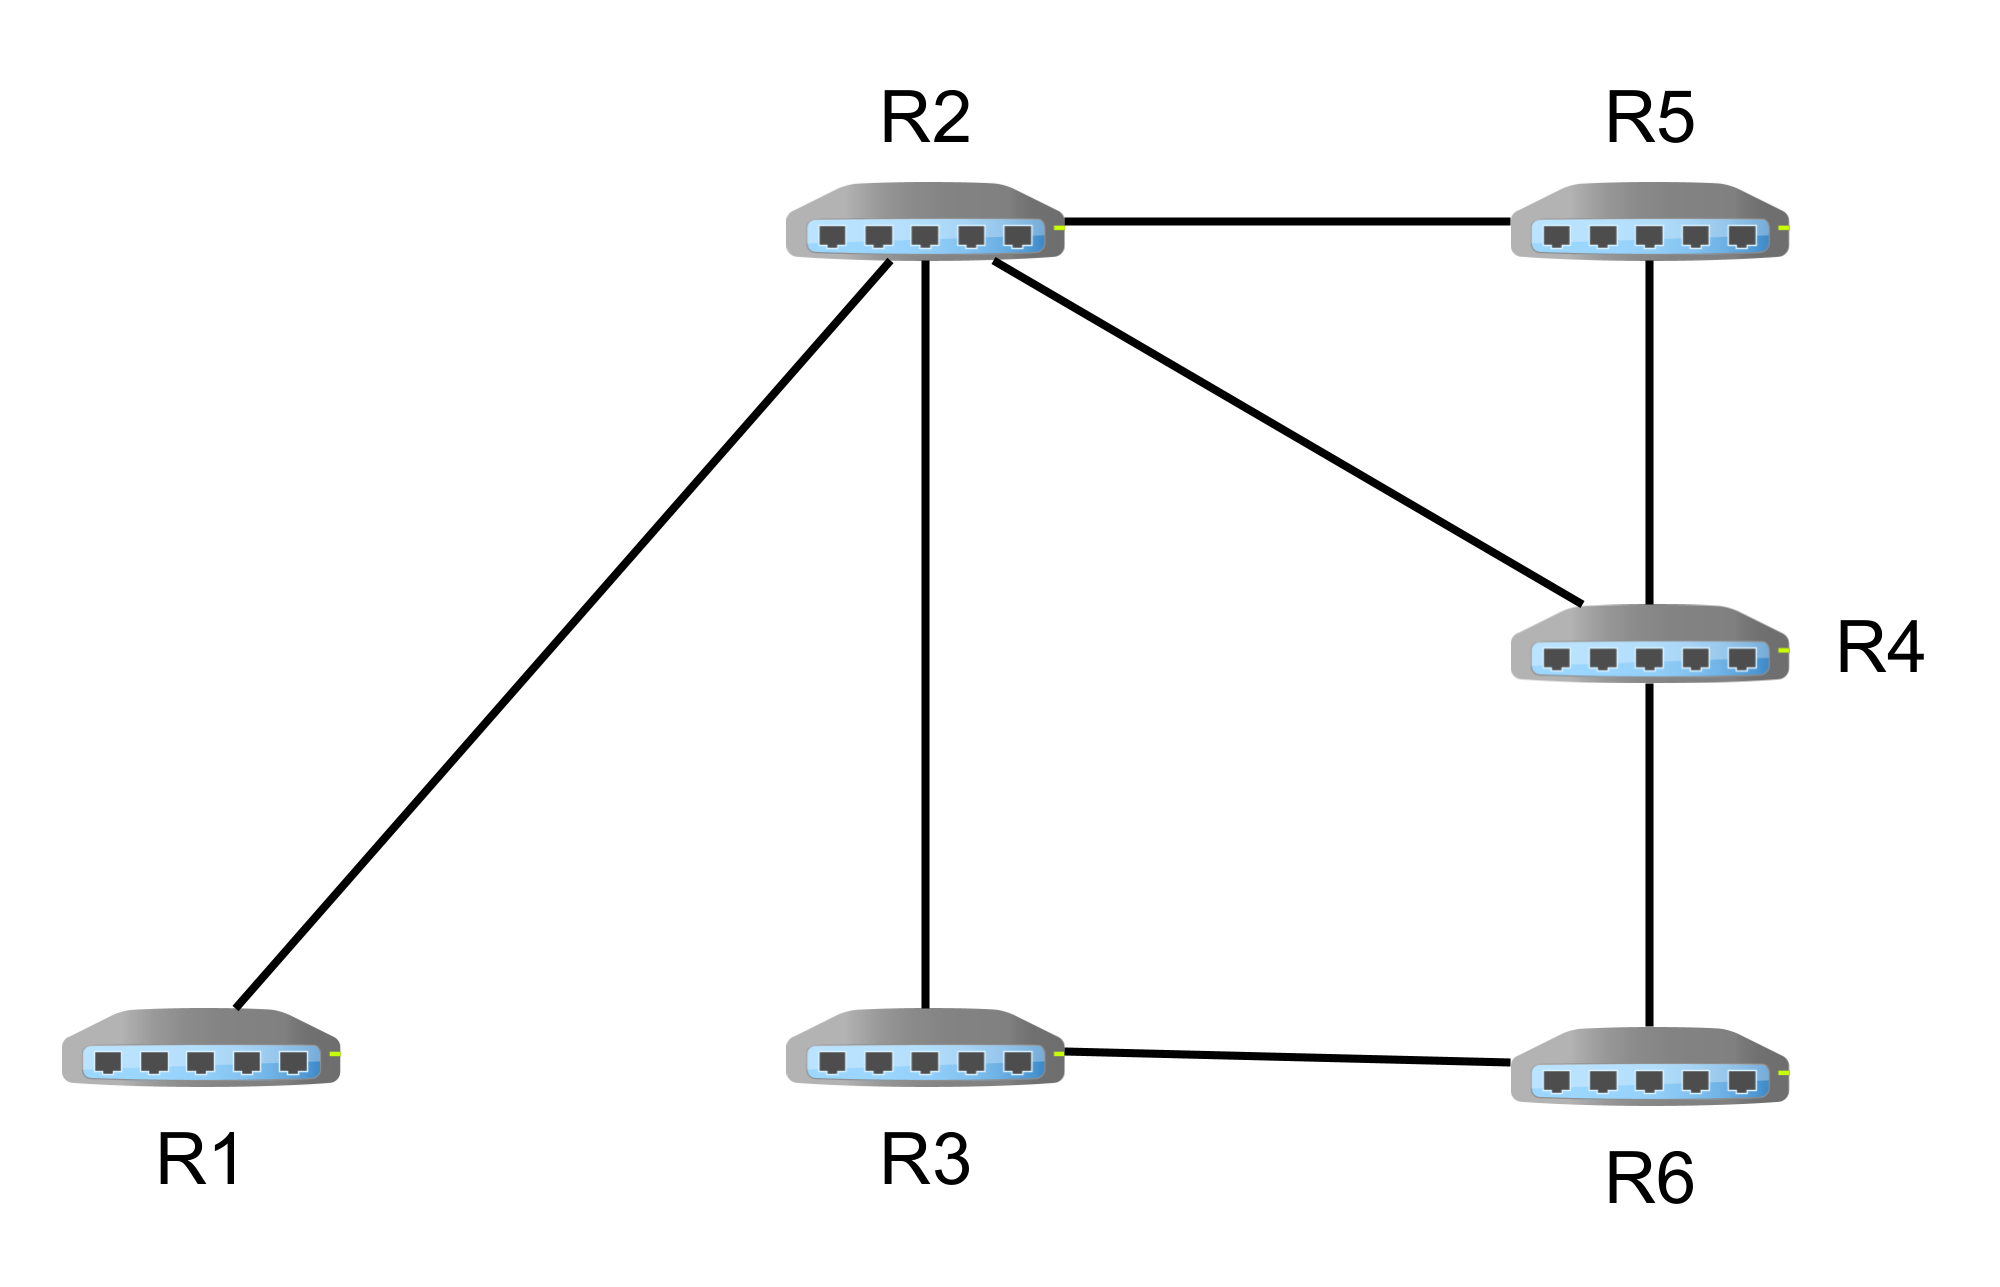
\includegraphics[width=6cm]{img/res1.png}
\end{center}

Donner étape par étape l'évolution des tables de routage de R1 et R6.\\
On n'indique pas les IP, juste les routeurs (c'est souvent ainsi lors du baccalauréat), par exemple au départ, R2 est à distance 1 de R1 en passant par... R1.
\end{exercice}

\begin{exercice}[ : Effet d'une panne]
	On considère le réseau suivant
	\begin{center}
		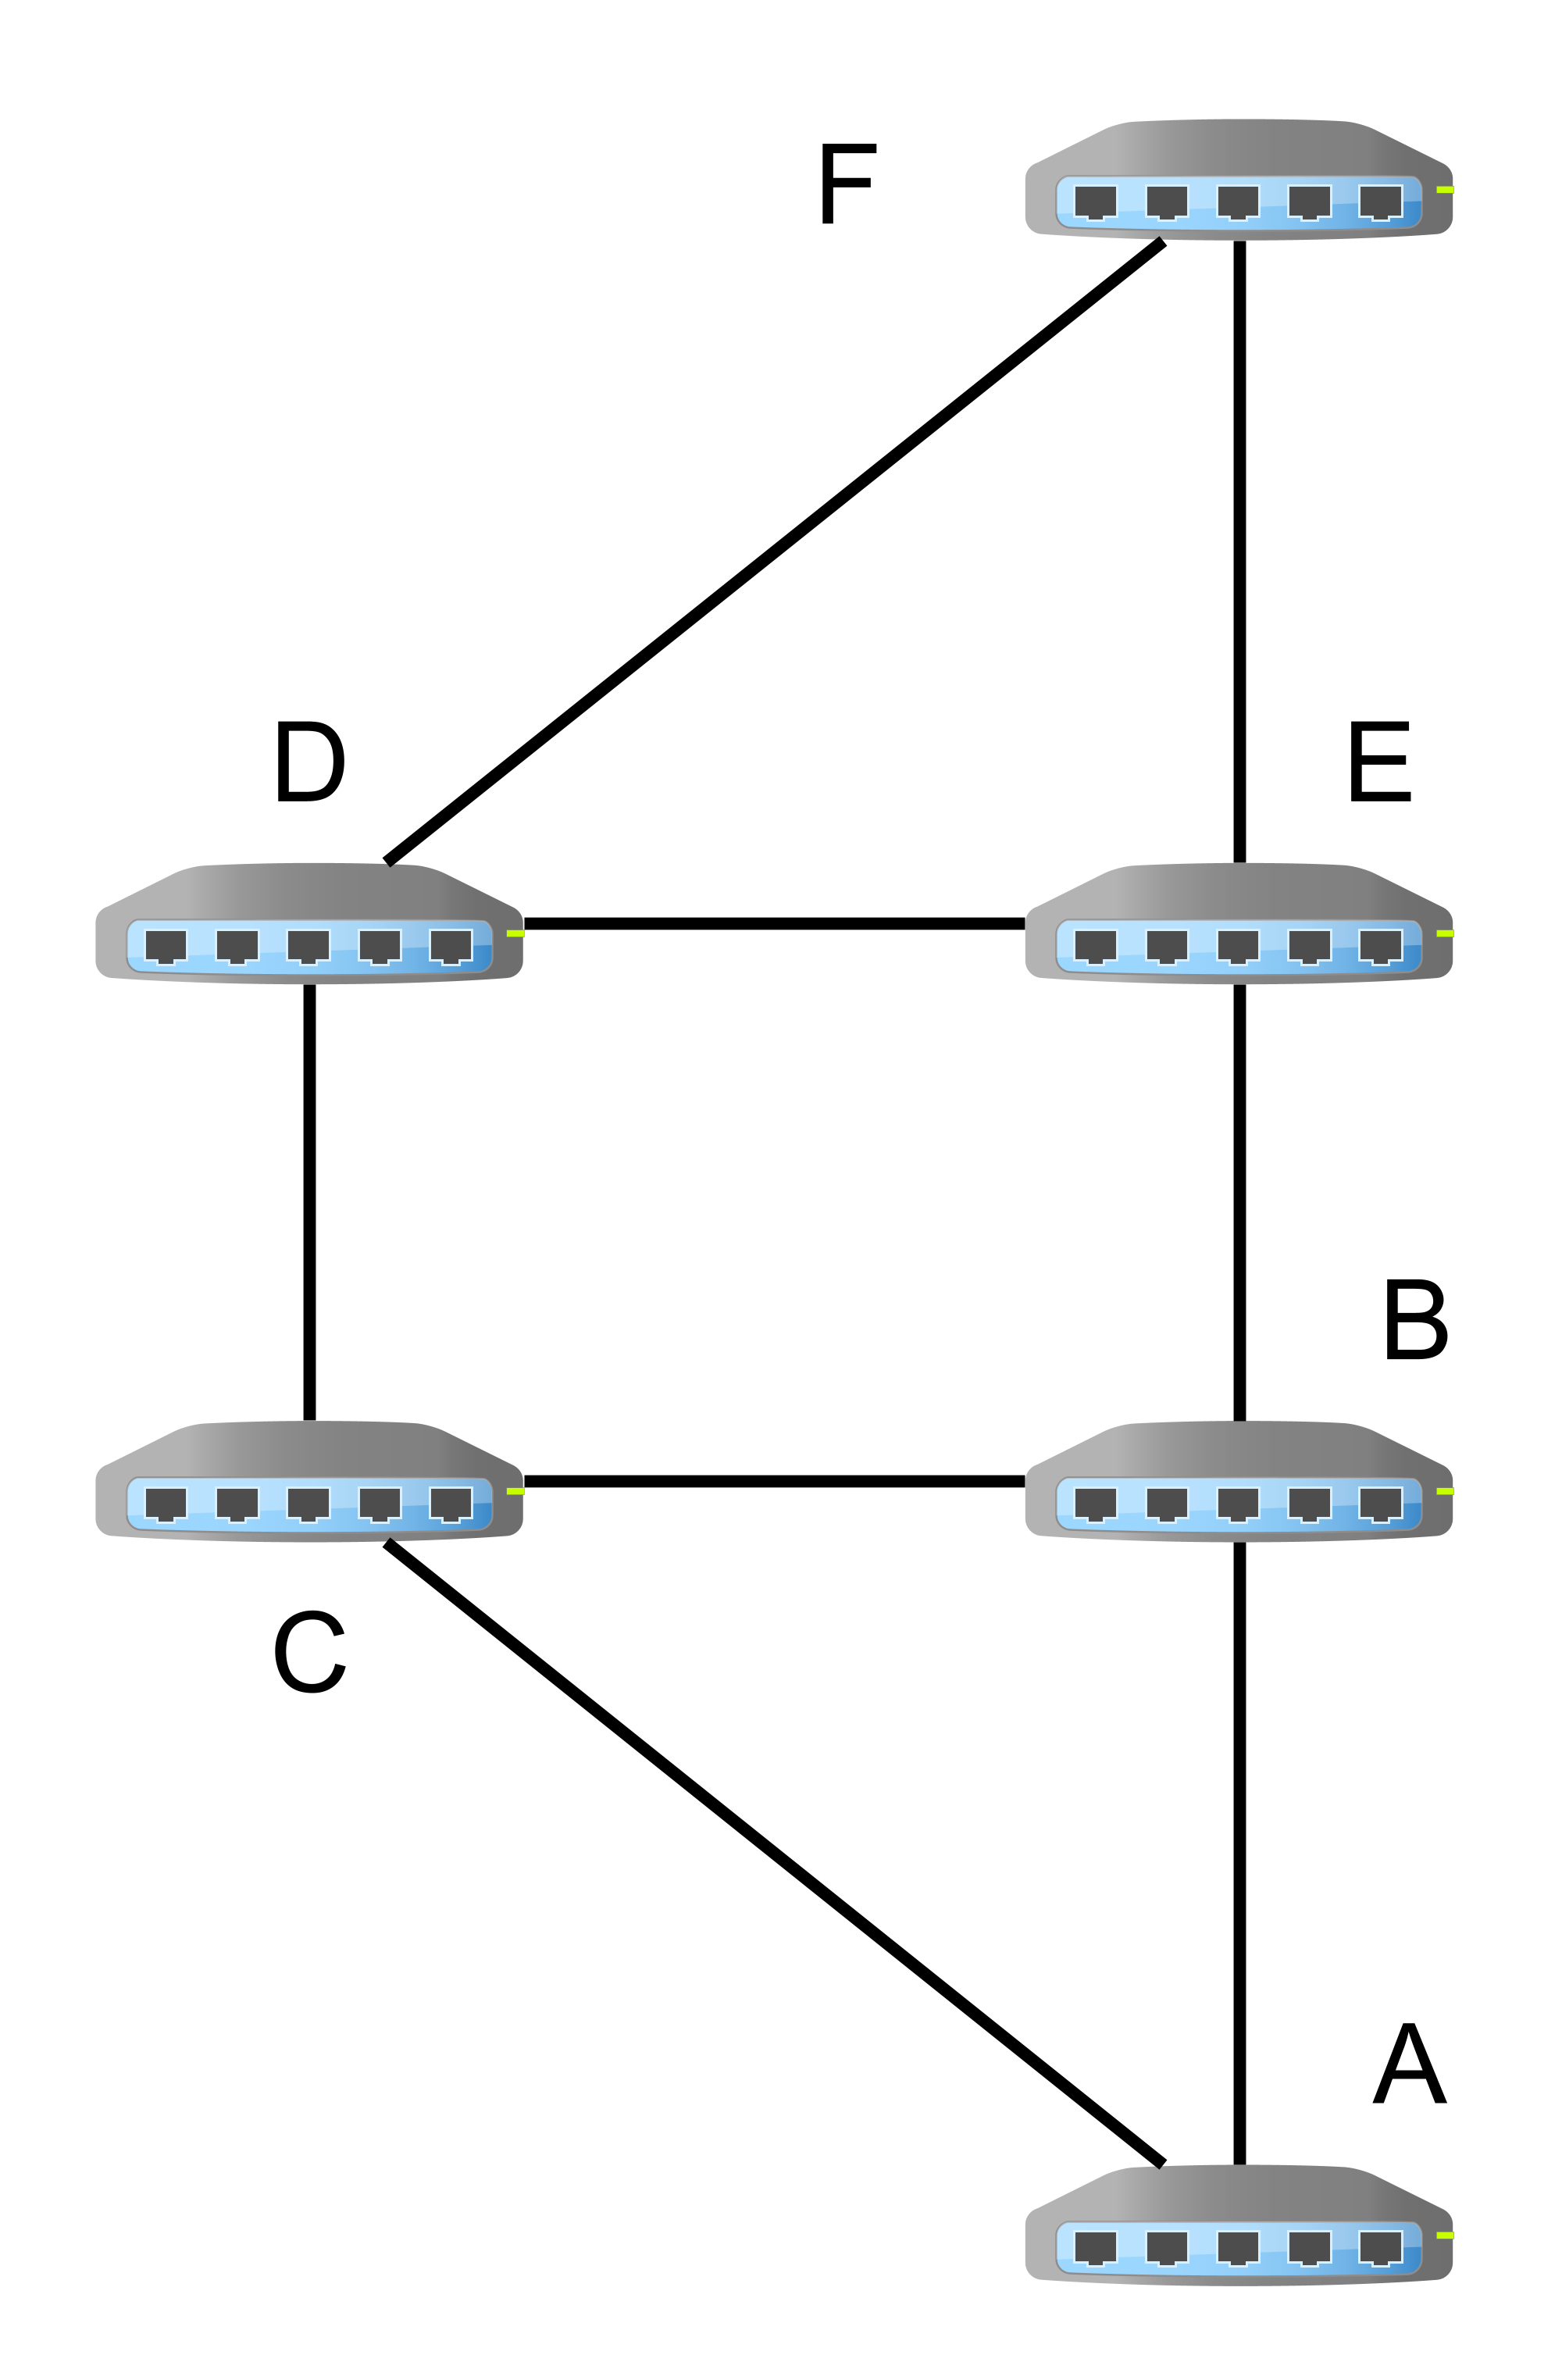
\includegraphics[width=6cm]{img/res2.png}
	\end{center}

\newpage 

\begin{enumerate}
	\item Remplir la table de routage de A après convergence de RIP.
\begin{center}
\begin{tabular}{|c|c|c|}
	\hline
\rowcolor{UGLiOrange}	\textbf{\color{white}Destination} & \textbf{\color{white}Distance} & \textbf{\color{white}Intermédiaire} \\	\hline
	B &  &  \\
	\hline
	C &  &  \\
	\hline
	D &  &  \\
	\hline
	E &  &  \\
	\hline
	F &  &  \\
	\hline
\end{tabular}

\end{center}
	\item Le routeur B tombe en panne : il n'émet plus de message RIP.\\
Que va-t-il se passer et comment va évoluer la table de routage de A ?
\end{enumerate}
\end{exercice}

\end{document}